\chapter{Results}
\textit{The data analysis is divided in to three different approaches. These methods follow the chronological evolution of the data analysis. The first method involves doing a simple paired t-test as on each frequency band. The second approach is mapping t-values as an image, to identify visual areas of activity in time. Lastly a ANOVA test is used as a verification of the two prior results.}

\section{Mean value test}

In line with the initial approach stated in the method section, a paired t-test combining the subject difference in two states of the experiment, has been carried out. The approach builds on using the total mean of each frequency band, condensing these down to just one number. The approach found no combination of regions and bands, that show a significant difference between subject in cuffed or uncuffed states. A table showing the tests p-values is show below in \cref{my:pval}.     


\begin{table}[H]
	\centering
	\caption{Table showing the different P-values corresponding to each region and frequency band}
	\scalebox{0.8}{
	\label{my:pval}
	\begin{tabular}{|l|l|l|l|}
		\hline
		& P-endo & P-myo  & P-neuro \\ \hline
		Region 10 & 0.7116 & 0.8454 & 0.9389  \\ \hline
		Region 14 & 0.6254 & 0.9237 & 0.6955  \\ \hline
		Region 20 & 0.4141 & 0.9237 & 0.8004  \\ \hline
		Region 21 & 0.4062 & 0.9564 & 0.8452  \\ \hline
		Region 22 & 0.3826 & 0.9323 & 0.1552  \\ \hline
	\end{tabular}}
\end{table}

Knowing 

\section{T-value mapping}
Results of the data analysis, as illustrated on fig, shows a t-tested image from a summation of all scalograms within the two conditions for each region. The y-axis shows the number of different frequencies and the x-axis is time, giving in number of frames. Each pixel within the final image has a t-value corresponding to the test of the uncuffed pixel value compared to the cuffed pixel value. The larger t-value, the brighter a pixel will appear in the image. The image showed no areas where a greater difference could be observed. Mostly individual pixels lid up showing a great difference, but as these are individual and not part of an area, these are considered outliers.  

\begin{figure}[H]
	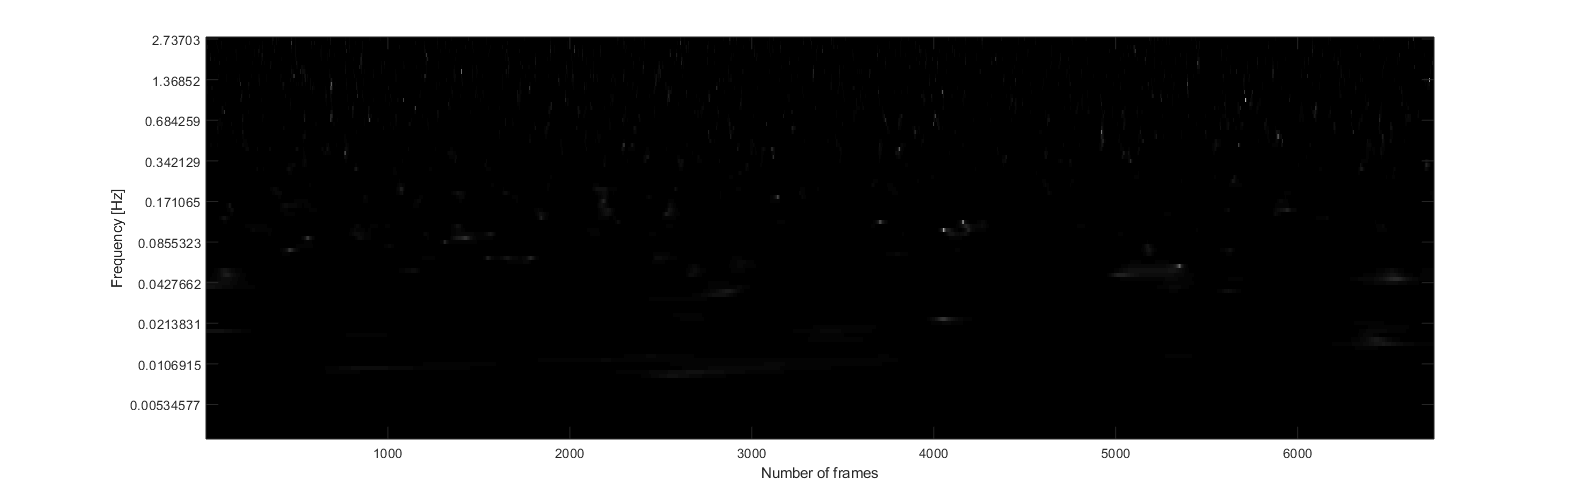
\includegraphics[width=1\textwidth]{figures/t-values_roi10}
	\caption{The original data of region 15 in the uncuffed recording of subject 1 including 20 jumps.}
	\label{fig:raw15}
\end{figure}

Neither of the images corresponding to each region showed areas where vasomotion activity could be identified. The remaining t-value mapping images can be seen in \cref{t-value}.  
The number of positive and negative t-values for each frequency band in every region is compared in \cref{tab:t}. Positive t-values indicate a drop in amplitude from the uncuffed state to the cuffed and negative values the opposite. No  
\begin{table}[H]
	\centering
	\caption{Table with comparison of t-values for every band at every region.}
	\label{tab:t}
	\scalebox{0.7}{
	\begin{tabular}{|l|l|l|l|}
		\hline
		& Endo band      & Neuro band     & Myo band       \\ \hline
		\multicolumn{4}{|l|}{Region 10}                                         \\ \hline
		Positive vs negative & 67704 vs 74025 & 49383 vs 38354 & 54145 vs 53839 \\ \hline
		\multicolumn{4}{|l|}{Region 14}                                         \\ \hline
		Positive vs negative & 76377 vs 65352 & 49665 vs 38072 & 55092 vs 52892 \\ \hline
		\multicolumn{4}{|l|}{Region 20}                                         \\ \hline
		Positive vs negative & 79309 vs 62428 & 44248 vs 43489 & 52116 vs 55968 \\ \hline
		\multicolumn{4}{|l|}{Region 21}                                         \\ \hline
		Positive vs negative & 74634 vs 67095 & 43542 vs 44195 & 52941 vs 55043 \\ \hline
		\multicolumn{4}{|l|}{Region 22}                                         \\ \hline
		Positive vs negative & 88601 vs 53128 & 64195 vs 23542 & 51462 vs 56522 \\ \hline
	\end{tabular}}
\end{table}
%T is simply the calculated difference represented in units of standard error. The greater the magnitude of T (it can be either positive or negative), the greater the evidence against the null hypothesis that there is no significant difference. The closer T is to 0, the more likely there isn't a significant difference.

\section{ANOVA}